% Informe final — Lab 7, Automatización, Universidad Católica
% Proyecto independiente, con registros de los cuatro ensayos experimentales.
\documentclass[conference,10pt,letterpaper]{IEEEtran}
\usepackage[T1]{fontenc}
\usepackage[utf8]{inputenc}
\usepackage[spanish,es-nodecimaldot]{babel}
\usepackage{mathptmx}
\usepackage{amsmath,amssymb,mathtools}
\usepackage{graphicx}
\usepackage{booktabs,tabularx,array,multirow}
\usepackage{cite}
\usepackage{xurl}
\usepackage[hidelinks]{hyperref}
\usepackage{siunitx}
\usepackage{microtype}
\usepackage{balance}
\usepackage{fancyhdr}
% Firma de cierre exclusivamente en la ultima pagina del documento.
\fancypagestyle{sdgultima}{%
  \fancyhf{}%
  \fancyfoot[C]{\thepage}%
  \fancyfoot[R]{\normalfont\footnotesize SDG}%
  \renewcommand{\headrulewidth}{0pt}%
  \renewcommand{\footrulewidth}{0pt}%
}
\AtEndDocument{\thispagestyle{sdgultima}}
\usepackage{placeins}
\sisetup{output-decimal-marker={,},group-separator={\,},group-minimum-digits=4}
\graphicspath{{figuras/}}
\setlength{\textfloatsep}{8pt plus 2pt minus 3pt}
\setlength{\floatsep}{7pt plus 2pt minus 2pt}
\setlength{\intextsep}{8pt plus 2pt minus 2pt}
\title{Control digital por realimentación de estados estimados:\\ diseño e implementación de observadores de predicción y estado actual}
\author{\IEEEauthorblockN{Aldo Pastore}
\IEEEauthorblockA{Automatización -- Ingeniería Electrónica\\
Facultad de Ciencias y Tecnología\\
Universidad Católica ``Nuestra Señora de la Asunción'' -- Asunción, Paraguay\\
\texttt{aldo.pastore@uc.edu.py}}}
\begin{document}
\maketitle
\begin{abstract}
Se diseñaron e implementaron cuatro configuraciones de control digital por realimentación de estados estimados sobre una planta analógica de segundo orden. Se compararon observadores de predicción y de estado actual mediante dos ubicaciones de polos, manteniendo el controlador y el escalón de referencia de \SI{50}{\milli\volt} comunes. La planta se discretizó con retenedor de orden cero y un período de \SI{2}{\milli\second}; la discrepancia entre el modelo nominal y el identificado previamente obligó a rediseñar E1 antes de la implementación física, mientras que E2 conservó su asignación original. En un PSoC 5LP se registraron 256 muestras por ensayo y simultáneamente se midieron el mando en J5 y la salida en J7 con un Rigol DS1202Z-E. Los cuatro ensayos concluyeron sin banderas de error, con sobrepasamientos de 20 a 30\,\% y picos nominales de mando de \SI{92}{\milli\volt}. El valor medio final informado por el ADC se situó entre \SI{43,12}{\milli\volt} y \SI{47,88}{\milli\volt}; no obstante, los incrementos físicos de la salida medidos por el osciloscopio se agruparon entre \SI{44,33}{\milli\volt} y \SI{44,74}{\milli\volt}. Esta diferencia evidencia la influencia del cero de adquisición y la cuantización en la comparación del seguimiento. Se documentan asimismo las limitaciones de sincronización y alcance de la validación.
\end{abstract}
\begin{IEEEkeywords}
control digital, observador de estados, estimador de predicción, estimador actual, ubicación de polos, cuantización, PSoC 5LP.
\end{IEEEkeywords}

\section{Objetivos y alcance}
La práctica consistió en cerrar el lazo de una planta de dos etapas mediante realimentación de estados que no se miden en forma independiente. Se compararon dos secuencias de estimación: la corrección de predicción, que afecta al estado de la muestra siguiente, y la corrección actual, que utiliza la medida disponible antes de calcular la acción de control. En cada arquitectura se estudiaron dos ubicaciones de polos del observador. Se conservaron el período de muestreo, la ley de realimentación y la referencia para distinguir el efecto de la estructura de estimación de las variaciones del experimento.

El informe reúne el diseño matemático, la evaluación de estabilidad frente a la planta identificada, la implementación en PSoC y cuatro ensayos físicos sobre el mismo circuito. Se distinguen las magnitudes previstas en MATLAB, los valores discretos comunicados por el microcontrolador y las tensiones continuas registradas por el osciloscopio; esta distinción es indispensable al estudiar control digital con muestreo y retención \cite{samanta2024,fadali2020}.

\section{Modelo de la planta}
\subsection{Representación continua}
La planta consta de dos etapas inversoras de primer orden. Para los estados asociados a sus salidas internas, \(x_1\) y \(x_2\), se escribe
\begin{equation}
 \dot{\boldsymbol{x}}(t)=F\boldsymbol{x}(t)+Gu(t),\qquad
 y(t)=H\boldsymbol{x}(t),
 \label{eq:continuo}
\end{equation}
con \(\boldsymbol{x}=[x_1\;x_2]^T\), \(H=[0\;1]\) y \(J=0\). A partir de los valores nominales del circuito, \(R_5=150\,\mathrm{k}\Omega\), \(R_6=47\,\mathrm{k}\Omega\), \(R_1=15\,\mathrm{k}\Omega\), \(R_2=47\,\mathrm{k}\Omega\), \(C_1=C_3=100\,\mathrm{nF}\), se tienen
\begin{equation}
F=\begin{bmatrix}
-\frac{1}{R_5 C_1} & 0\\
-\frac{1}{R_2 C_3} & -\frac{1}{R_1 C_3}
\end{bmatrix},\qquad
G=\begin{bmatrix}-\frac{1}{R_6 C_1}\\0\end{bmatrix}.
\label{eq:nominal_matrices}
\end{equation}
La doble inversión genera una ganancia estática positiva. El modelo nominal se conservó para desarrollar las matrices de control, pero no se consideró suficiente para representar por sí solo toda la respuesta física.

\subsection{Modelo identificado experimentalmente}
Para evaluar el comportamiento del montaje real se empleó el siguiente modelo, obtenido por identificación experimental de la respuesta temporal de la planta:
\begin{equation}
 G_{\mathrm{id}}(s)=\frac{1{,}002941}{(1+0{,}00906915s)(1+0{,}000774399s)}.
\label{eq:planta_id}
\end{equation}
Se obtienen dos constantes de tiempo muy distintas: \(\tau_1=\SI{9,06915}{\milli\second}\) y \(\tau_2=\SI{0,774399}{\milli\second}\). La segunda etapa concentra el polo de mayor rapidez. Esta diferencia entre parámetros nominales y experimentales resulta relevante cuando se trasladan al hardware ganancias diseñadas sobre el circuito ideal.

\subsection{Selección del muestreo y modelo discreto}
Se eligió \(T_s=\SI{2}{\milli\second}\), correspondiente a \(f_s=\SI{500}{\hertz}\) y \(\omega_s=\SI{3141,59}{\radian\per\second}\). Respecto a la frecuencia característica de diseño \(\omega_n=\SI{360}{\radian\per\second}\), el cociente es \(\omega_s/\omega_n=8{,}73\), superior al criterio mínimo de ocho empleado en la guía \cite{guiaLab7}. La elección se realizó antes de discretizar, de acuerdo con las consideraciones sobre muestreo y retenedor de orden cero de \cite{samanta2024,fadali2020}.

En condiciones de mando constante durante cada intervalo,
\begin{equation}
 A=e^{FT_s},\qquad B=\int_0^{T_s}e^{F\tau}G\,\mathrm{d}\tau,
 \quad C=H,\quad D=0.
 \label{eq:zoh}
\end{equation}
Para el modelo nominal y la base de estados anterior, MATLAB entregó
\begin{equation}
 A=\begin{bmatrix}0{,}8752&0\\-0{,}2169&0{,}2636\end{bmatrix},\quad
 B=\begin{bmatrix}-0{,}3984\\0{,}0579\end{bmatrix},\quad C=[0\;1].
 \label{eq:AB}
\end{equation}
Las matrices de controlabilidad \(\mathcal C=[B\;AB]\) y observabilidad \(\mathcal O=[C^T\;(CA)^T]^T\) tienen rango dos. Por consiguiente, ambos estados son controlables y observables desde la única salida utilizada.

\section{Controlador y diseño de los estimadores}
\subsection{Realimentación y referencia}
Los polos del controlador se asignaron a \(0{,}80\pm j0{,}25\), dentro del círculo unidad. La ley digital fue
\begin{equation}
 u[k]=-K\widehat{\boldsymbol{x}}_u[k]+N_r r[k],\quad
 K=\begin{bmatrix}2{,}1569&6{,}8713\end{bmatrix},
 \label{eq:control}
\end{equation}
con \(N_r=1{,}09474803\). El símbolo \(\widehat{\boldsymbol{x}}_u\) representa el estado estimado efectivamente empleado por la ley de control; su definición depende del observador. Para una planta SISO sin paso directo, el precompensador se obtiene de
\begin{equation}
 N_r=\bigl[C(I-A+BK)^{-1}B\bigr]^{-1}.
 \label{eq:nr}
\end{equation}
La precompensación asegura seguimiento unitario en el modelo lineal nominal y sin cuantización, pero no elimina por sí misma el error de seguimiento en una implementación con mandos discretos, incertidumbre paramétrica y calibración del ADC \cite{fadali2020,astrom2020}.

\subsection{Estimador de predicción}
El observador predictor utiliza, en el instante \(k\), la estimación disponible antes de la corrección con la muestra actual:
\begin{align}
 \nu[k]&=y[k]-C\widehat{\boldsymbol{x}}^-[k],\\
 u[k]&=-K\widehat{\boldsymbol{x}}^-[k]+N_r r[k],\\
 \widehat{\boldsymbol{x}}^-[k+1]&=A\widehat{\boldsymbol{x}}^-[k]
       +Bu[k]+L_p\nu[k].
\label{eq:pred}
\end{align}
La matriz de error del predictor ideal es \(A-L_pC\). La corrección calculada con \(y[k]\) influye sobre el control a partir de la muestra siguiente.

\subsection{Estimador de estado actual}
En el estimador actual, la innovación modifica el estado antes de calcular el mando:
\begin{align}
 \widehat{\boldsymbol{x}}^+[k]&=\widehat{\boldsymbol{x}}^-[k]+L_a\nu[k],\\
 u[k]&=-K\widehat{\boldsymbol{x}}^+[k]+N_r r[k],\\
 \widehat{\boldsymbol{x}}^-[k+1]&=A\widehat{\boldsymbol{x}}^+[k]+Bu[k].
 \label{eq:actual}
\end{align}
La dinámica del error corregido se asocia a \((I-L_aC)A\). Por esta razón, las ganancias del observador actual no son intercambiables con las del predictor, aunque ambas arquitecturas compartan el mismo controlador \(K\) \cite{samanta2024,fadali2020}.

\subsection{Ubicación de polos y rediseño de E1}
La guía propone dos parejas de polos para los observadores, E1: \(0{,}40\pm j0{,}25\) y E2: \(0{,}20\pm j0{,}10\). El cálculo sobre la planta nominal no reveló inestabilidad. Sin embargo, al evaluar el sistema aumentado con la planta identificada, el observador actual E1 original alcanzó un radio espectral de \(1{,}0487\); por ello no se llevó esa configuración original al circuito.

Se exploró una ubicación más amortiguada, \(0{,}35\pm j0{,}10\), para E1. La nueva pareja de ganancias conservó el mismo \(K\) y redujo el radio espectral del modelo aumentado por debajo de la unidad. E2 no requirió ese cambio. En adelante, las denominaciones \emph{E1 alternativo} y \emph{E2 original} distinguen diseños físicamente diferentes.

\begin{table}[!t]
\caption{Ganancias de estimación implementadas en el PSoC}
\label{tab:ganancias}
\centering\footnotesize
\begin{tabular}{@{}llrr@{}}
\toprule
Polos & Estructura & $L_1$ & $L_2$\\
\midrule
$0{,}35\pm j0{,}10$ & Predictor E1 alt. & $-1{,}3179$ & $0{,}4388$\\
 & Actual E1 alt. & $-1{,}5058$ & $0{,}4256$\\
$0{,}20\pm j0{,}10$ & Predictor E2 orig. & $-2{,}1481$ & $0{,}7388$\\
 & Actual E2 orig. & $-2{,}4545$ & $0{,}7833$\\
\bottomrule
\end{tabular}
\end{table}

\begin{table}[!t]
\caption{Radio espectral del sistema aumentado sobre la planta identificada}
\label{tab:rho}
\centering\footnotesize
\begin{tabular}{@{}lcc@{}}
\toprule
Diseño & $\rho_{\mathrm{id}}$ & Estabilidad lineal\\
\midrule
Predictor E1 original & $0{,}9108$ & Sí\\
Actual E1 original & $1{,}0487$ & No\\
Predictor E1 alternativo & $0{,}8550$ & Sí\\
Actual E1 alternativo & $0{,}8737$ & Sí\\
Predictor E2 original & $0{,}8288$ & Sí\\
Actual E2 original & $0{,}8251$ & Sí\\
\bottomrule
\end{tabular}
\end{table}

El criterio \(\rho<1\) se refiere a la estabilidad asintótica del modelo \emph{lineal} aumentado en la condición evaluada. No reemplaza la comprobación de saturación, cuantización ni las mediciones físicas.

\section{Implementación digital y procedimiento}
\subsection{Arquitectura de adquisición y control}
Se utilizó una PCB analógica de segundo orden, con su salida acondicionada conectada al ADC SAR del PSoC 5LP y sus ramas DAC bipolares destinadas a generar el mando físico en J5. Un temporizador provoca la adquisición a \(T_s=2\,\mathrm{ms}\); la interrupción procesa la muestra, actualiza el estimador, calcula el mando y registra una fila de telemetría. La salida final de la planta se observa en J7. La implementación conserva 256 muestras por ensayo y 32 muestras iniciales de pretrigger, utilizadas para obtener el cero de la salida antes de aplicar la referencia.

La medición convertida se refiere a la salida mediante la calibración previa, mientras que la referencia \(r[k]\) y el control interno se expresan en voltios de la planta. La corrección previa del cero se aplica antes de ejecutar el observador, sin modificar posteriormente la amplitud de los registros. La referencia común fue \(r[k]=50\,\mathrm{mV}\) desde \(k=32\), es decir, \(t=64\,\mathrm{ms}\).

\subsection{Cuantización y protección}
La etapa bipolar presenta escalones nominales diferentes según el signo del mando. En el modelo de prevalidación se utilizaron incrementos aproximados de \(15{,}37\,\mathrm{mV}\) por código positivo y \(10{,}56\,\mathrm{mV}\) por código negativo. El firmware establece un intervalo conservador para el mando solicitado de \(-115\) a \(+107\,\mathrm{mV}\), y verifica códigos que no deben producir más de \(\pm120\,\mathrm{mV}\) nominales. El máximo aplicado por el DAC observado en las cuatro capturas fue \(92\,\mathrm{mV}\).

Se incorporaron banderas de rango del ADC, límite del mando, cálculo no finito, tiempo de CPU, irregularidad del intervalo y salida fuera de rango. Ante una condición detectada se ordena poner el DAC a cero y detener la adquisición. La revisión del código identificó que ciertas comprobaciones de CPU y del mando nominal se hacen después de la escritura física; por ello esta lógica constituye un mecanismo de parada, no una garantía absoluta de inexistencia de un transitorio breve.

\subsection{Instrumentación y sincronización}
Se conectó CH1 del Rigol DS1202Z-E a J5 y CH2 a J7; ambas sondas se configuraron en \(10\times\), acoplamiento DC y límite de banda de \SI{20}{\mega\hertz}. Se trabajó con \(50\,\mathrm{mV/div}\) en CH1, \(20\,\mathrm{mV/div}\) en CH2 y \(50\,\mathrm{ms/div}\). Un programa coordinó el anuncio de arranque por UART, el armado del osciloscopio y un disparo de respaldo temporizado. Se guardaron 1200 puntos por canal con un intervalo de \(0{,}5\,\mathrm{ms}\), junto con la pantalla y la telemetría completa.

Los cuatro registros útiles presentan un escalón reconocible en J5. Sin embargo, los metadatos consignan disparo forzado \texttt{TFOR} y no confirman un disparo físico por flanco. En consecuencia, las curvas del Rigol se alinearon de manera aproximada con el cruce del 50\,\% de CH1 para comparaciones visuales; no se atribuyen diferencias de fracciones de milisegundo a las estructuras.

\section{Prevalidación de E2 con no idealidades}
La estabilidad lineal de E2 se complementó con simulaciones de la planta identificada, ADC y DAC cuantizados, límites conservadores y parada del ensayo si el control solicitado excedía el rango. Se ejecutaron 20 realizaciones por estructura y nivel de ruido gaussiano supuesto, con \(\sigma=0\), 3 y \(10\,\mathrm{mV}\) RMS aplicado a la entrada de medición del modelo. Este ruido es un escenario hipotético y no equivale a una estimación experimental del ruido interno del ADC.

\begin{table}[!t]
\caption{Simulaciones de E2 con cuantización y ruido supuesto}
\label{tab:prevalidacion}
\centering\footnotesize
\begin{tabular}{@{}lccc@{}}
\toprule
Estructura & $\sigma=0$ & $\sigma=3$ & $\sigma=10$ mV\\
\midrule
Predictor E2 & $0/20$ & $0/20$ & $1/20$\\
Actual E2 & $0/20$ & $0/20$ & $1/20$\\
\bottomrule
\end{tabular}
\end{table}

La única parada en cada estructura ocurrió en la repetición 16, muestra \(k=35\), aproximadamente \(6\,\mathrm{ms}\) después del escalón, por \texttt{SATURACION\_SOLICITADA}. El mayor mando DAC aplicado hasta el corte fue \(107{,}59\,\mathrm{mV}\); no se registró, en este escenario, una superación del límite físico nominal. Ambas estructuras compartieron la misma realización de ruido para esa repetición. Estos 20 casos no permiten inferir una probabilidad de fallo de la instalación ni una robustez garantizada fuera de las condiciones ensayadas.

\section{Resultados experimentales}
\subsection{Criterios de evaluación}
La salida máxima se obtuvo de \(y_{\mathrm{rel}}[k]\) desde el primer valor no nulo de \(r[k]\). El sobrepasamiento se calculó respecto de la referencia común, \(M_p=(y_{\max}-50)/50\times100\), expresado en porcentaje. El tiempo hasta el pico se contó desde el escalón. Para reducir la sensibilidad a una cuenta aislada del ADC, el valor final se estimó mediante el promedio de las últimas 50 muestras, equivalente a \(100\,\mathrm{ms}\). Se informa el error medio \(e_f=50-\overline{y}_{50}\) y su porcentaje respecto de la referencia.

\begin{table*}[!t]
\caption{Resultados de las cuatro configuraciones implementadas (UART del PSoC)}
\label{tab:resultados_uart}
\centering\footnotesize
\begin{tabular}{@{}lcccccccc@{}}
\toprule
Configuración & $y_{\max}$ (mV) & $M_p$ (\%) & $t_p$ (ms) & $\overline y_{50}$ (mV) & $e_f$ (mV) & $|u|_{\max}$ (mV) & CPU máx. ($\mu$s) & Flags\\
\midrule
Predictor E1 alternativo & 60 & 20 & 12 & 46,24 & 3,76 & 92 & 112 & 0\\
Actual E1 alternativo & 65 & 30 & 14 & 43,12 & 6,88 & 92 & 110 & 0\\
Predictor E2 original & 61 & 22 & 12 & 45,00 & 5,00 & 92 & 112 & 0\\
Actual E2 original & 64 & 28 & 14 & 47,88 & 2,12 & 92 & 111 & 0\\
\bottomrule
\end{tabular}
\end{table*}

\begin{figure*}[!t]
\centering
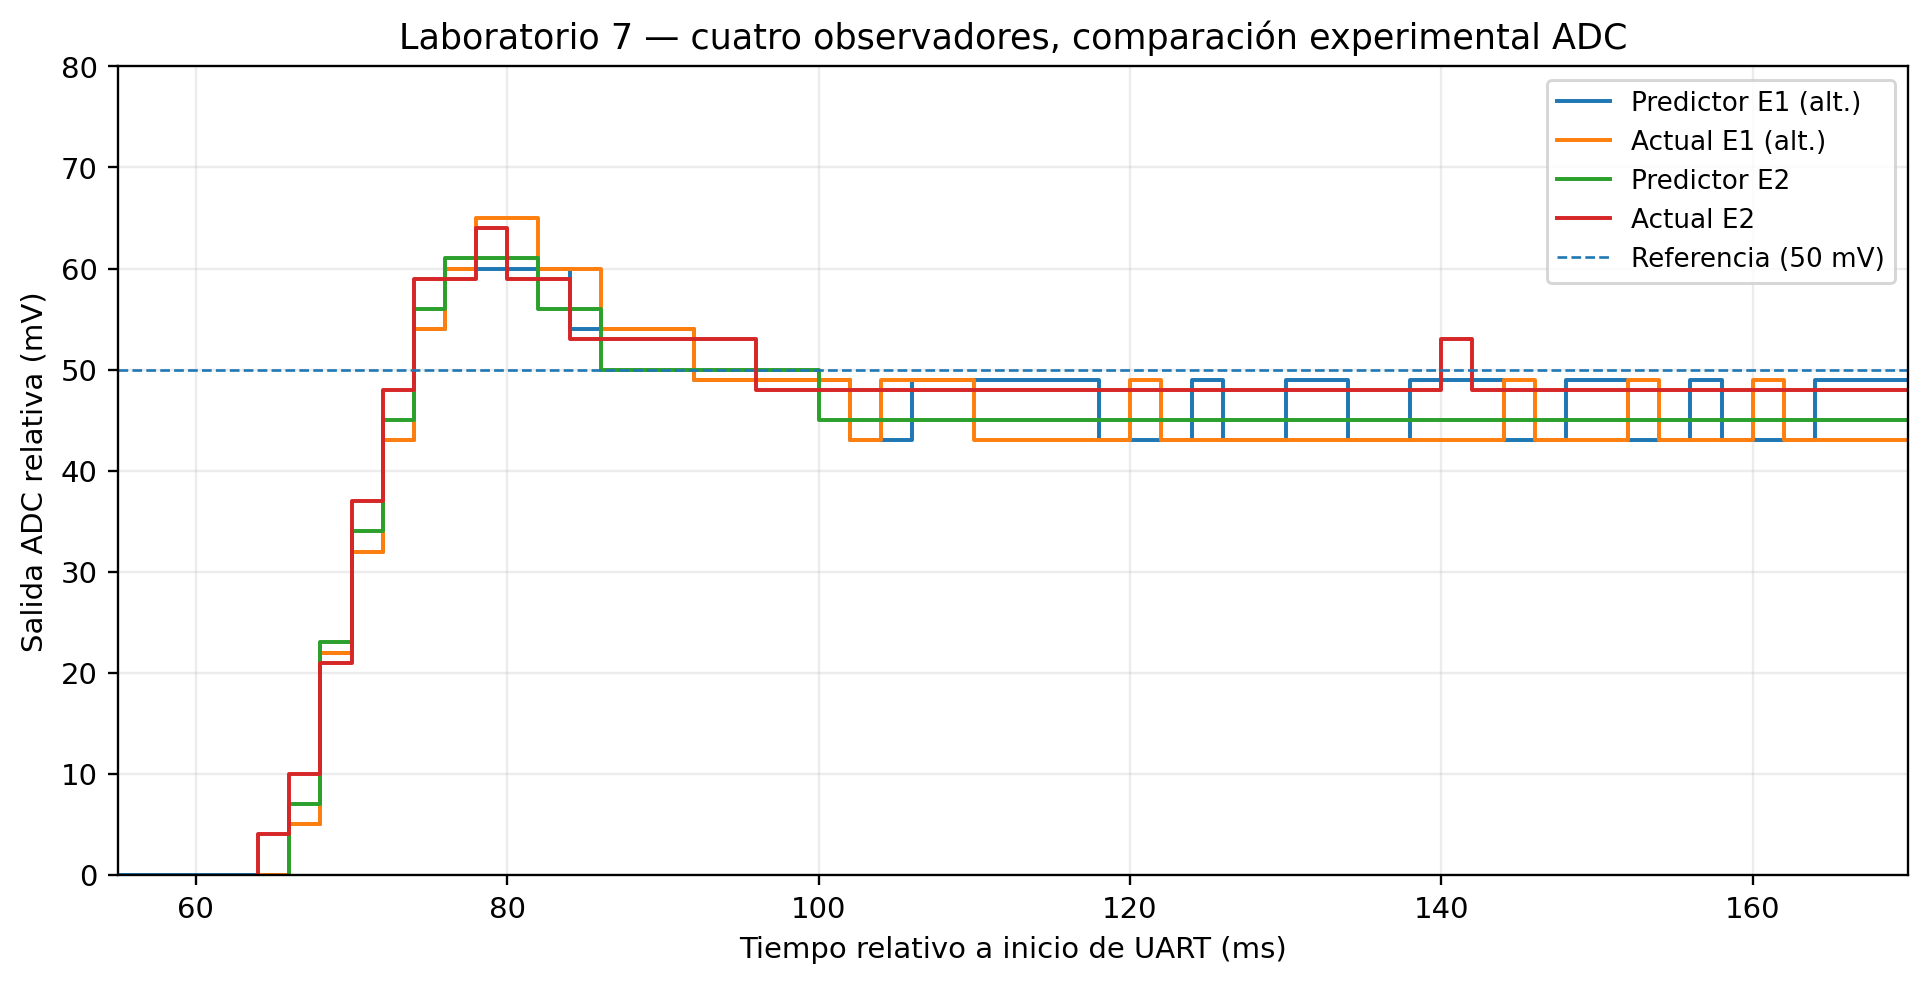
\includegraphics[width=0.94\textwidth]{07_cuatro_observadores_salida_ADC.png}
\caption{Comparación de las cuatro salidas discretas registradas por UART. Las curvas se alinean con el mismo instante programado de referencia de 50 mV y no han sido reescaladas para forzar coincidencia.}
\label{fig:cuatro_uart}
\end{figure*}

\begin{figure*}[!t]
\centering
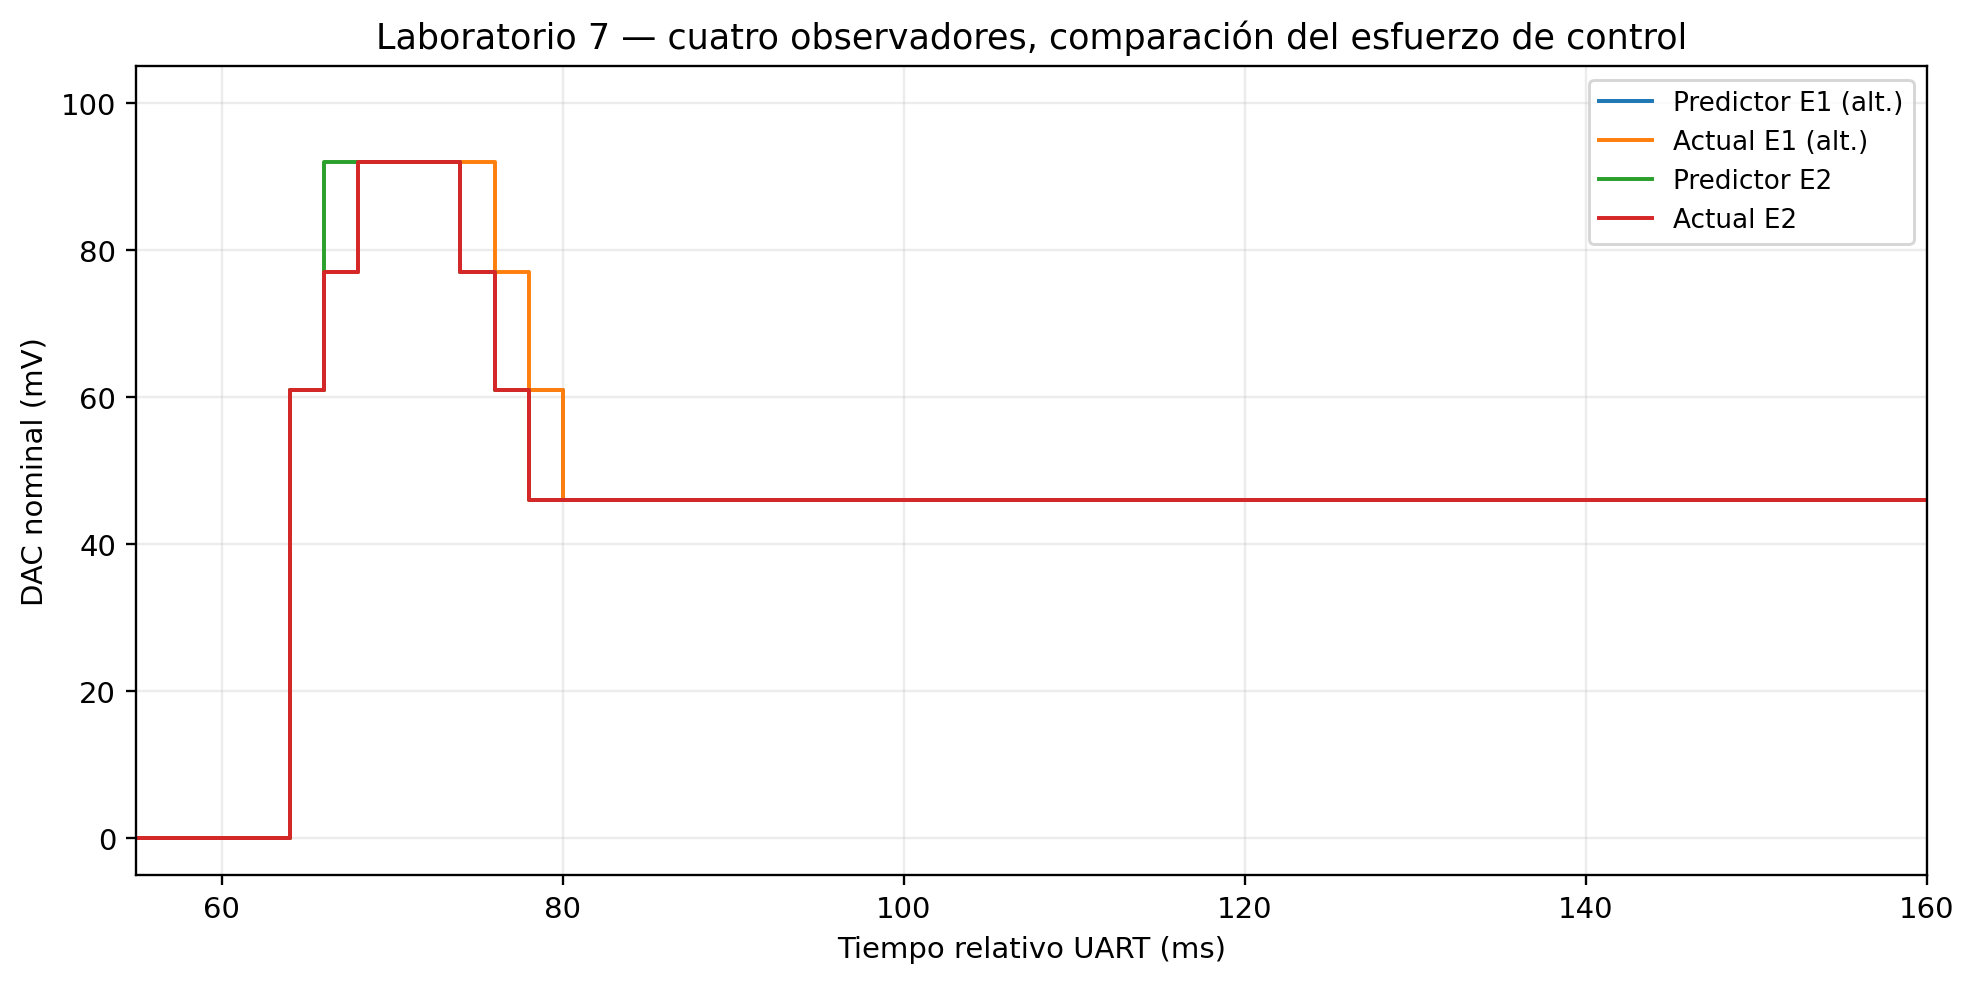
\includegraphics[width=0.94\textwidth]{08_cuatro_observadores_mando_DAC.png}
\caption{Mando nominal cuantizado de los cuatro controladores. La acción inicial alcanza 92 mV en todas las configuraciones; después de los transitorios se mantiene próxima a 46 mV.}
\label{fig:cuatro_dac}
\end{figure*}

La Tabla~\ref{tab:resultados_uart} y la Fig.~\ref{fig:cuatro_uart} muestran que los dos predictores alcanzaron picos de 60 y 61 mV, con 20 y 22\,\% de sobrepasamiento, mientras que los observadores actuales alcanzaron 65 y 64 mV, con 30 y 28\,\%. En esta ejecución, los predictores presentaron un transitorio ligeramente menos pronunciado. La diferencia no representa una superioridad general, pues no se ensayaron perturbaciones físicas independientes ni se repitieron suficientemente las mediciones.

En régimen, la media del Actual E2 quedó a 2,12 mV de la referencia, menor que los errores calculados por UART en los otros tres casos. El máximo de mando fue idéntico en las cuatro capturas (92 mV), de modo que las diferencias de pico no pueden atribuirse, en esta comparación, a una mayor amplitud máxima del DAC. La Fig.~\ref{fig:cuatro_dac} evidencia que el mismo actuador cuantizado limita la resolución del mando.

\subsection{Contraste con las señales físicas del osciloscopio}
Para cada canal del Rigol se obtuvo el promedio en reposo dentro de la ventana \((-250,-50)\,\mathrm{ms}\) y el promedio de meseta entre \(100\) y \(280\,\mathrm{ms}\) de su eje temporal. El incremento se calculó como diferencia entre ambas medias. Es distinto de la tensión absoluta, que incluye el nivel de cero de cada medición.

\begin{table}[!t]
\caption{Incrementos de tensión medidos por el Rigol en J5 y J7}
\label{tab:rigol}
\centering\footnotesize
\begin{tabular}{@{}lrr@{}}
\toprule
Configuración & $\Delta J5$ (mV) & $\Delta J7$ (mV)\\
\midrule
Predictor E1 alternativo & 45,19 & 44,74\\
Actual E1 alternativo & 45,35 & 44,69\\
Predictor E2 original & 44,96 & 44,49\\
Actual E2 original & 45,01 & 44,33\\
\bottomrule
\end{tabular}
\end{table}

\begin{figure*}[!t]
\centering
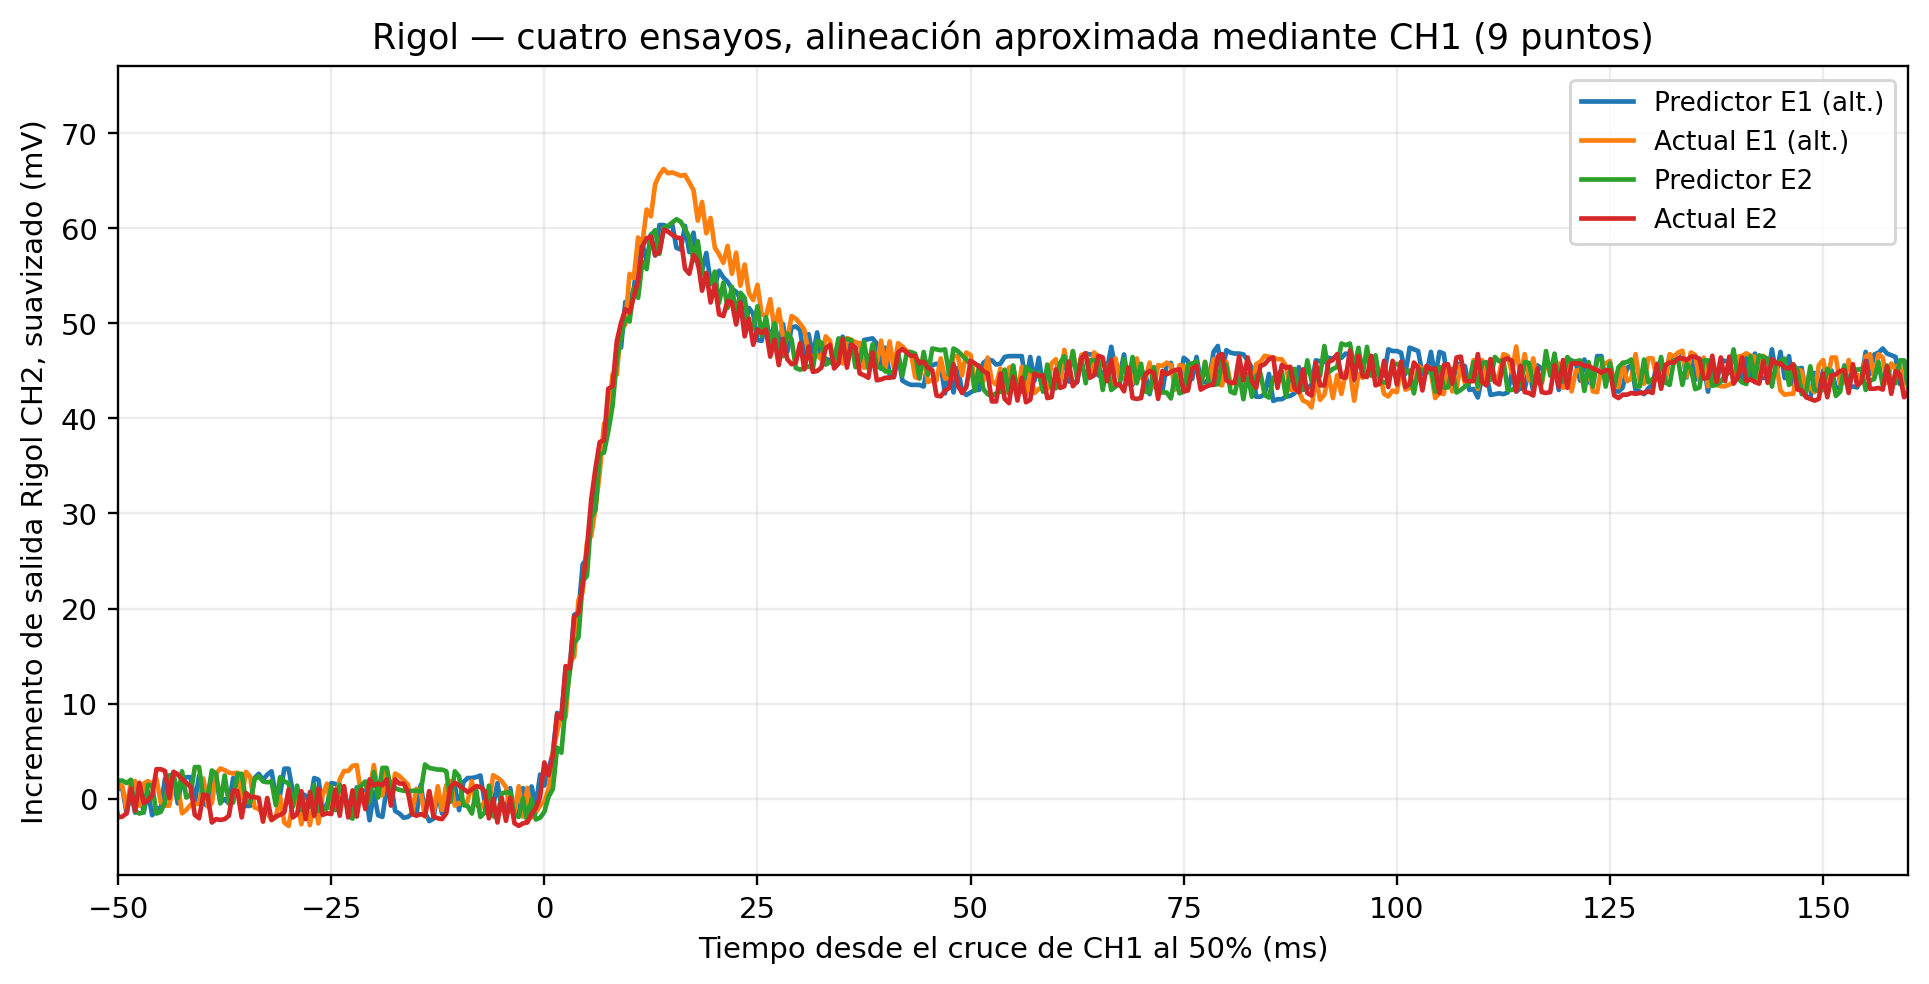
\includegraphics[width=0.96\textwidth]{10_cuatro_observadores_Rigol_CH2.png}
\caption{Respuesta física de J7 en los cuatro ensayos. Se ha restado el nivel medio de reposo y se aplica una media móvil de nueve puntos (4,5 ms) únicamente para legibilidad; el alineamiento por CH1 es aproximado porque el disparo fue temporizado.}
\label{fig:cuatro_rigol}
\end{figure*}

Los valores de la Tabla~\ref{tab:rigol} muestran que las cuatro salidas físicas se agrupan entre 44,33 y 44,74 mV. La separación máxima es de apenas 0,41 mV, muy inferior a la dispersión instantánea de aproximadamente 11,4--11,6 mV registrada en las mesetas de CH2. Los promedios de UART, en cambio, se separan hasta 4,76 mV. La diferencia revela la importancia de la calibración, el punto de referencia de cero y la cuantización en la interpretación de la salida discreta. Las cuatro señales físicas son muy parecidas al alcanzar su meseta, aun cuando el valor medio registrado por el ADC no coincide exactamente.

\subsection{Ejecución y error de estimación}
\begin{figure}[!t]
\centering
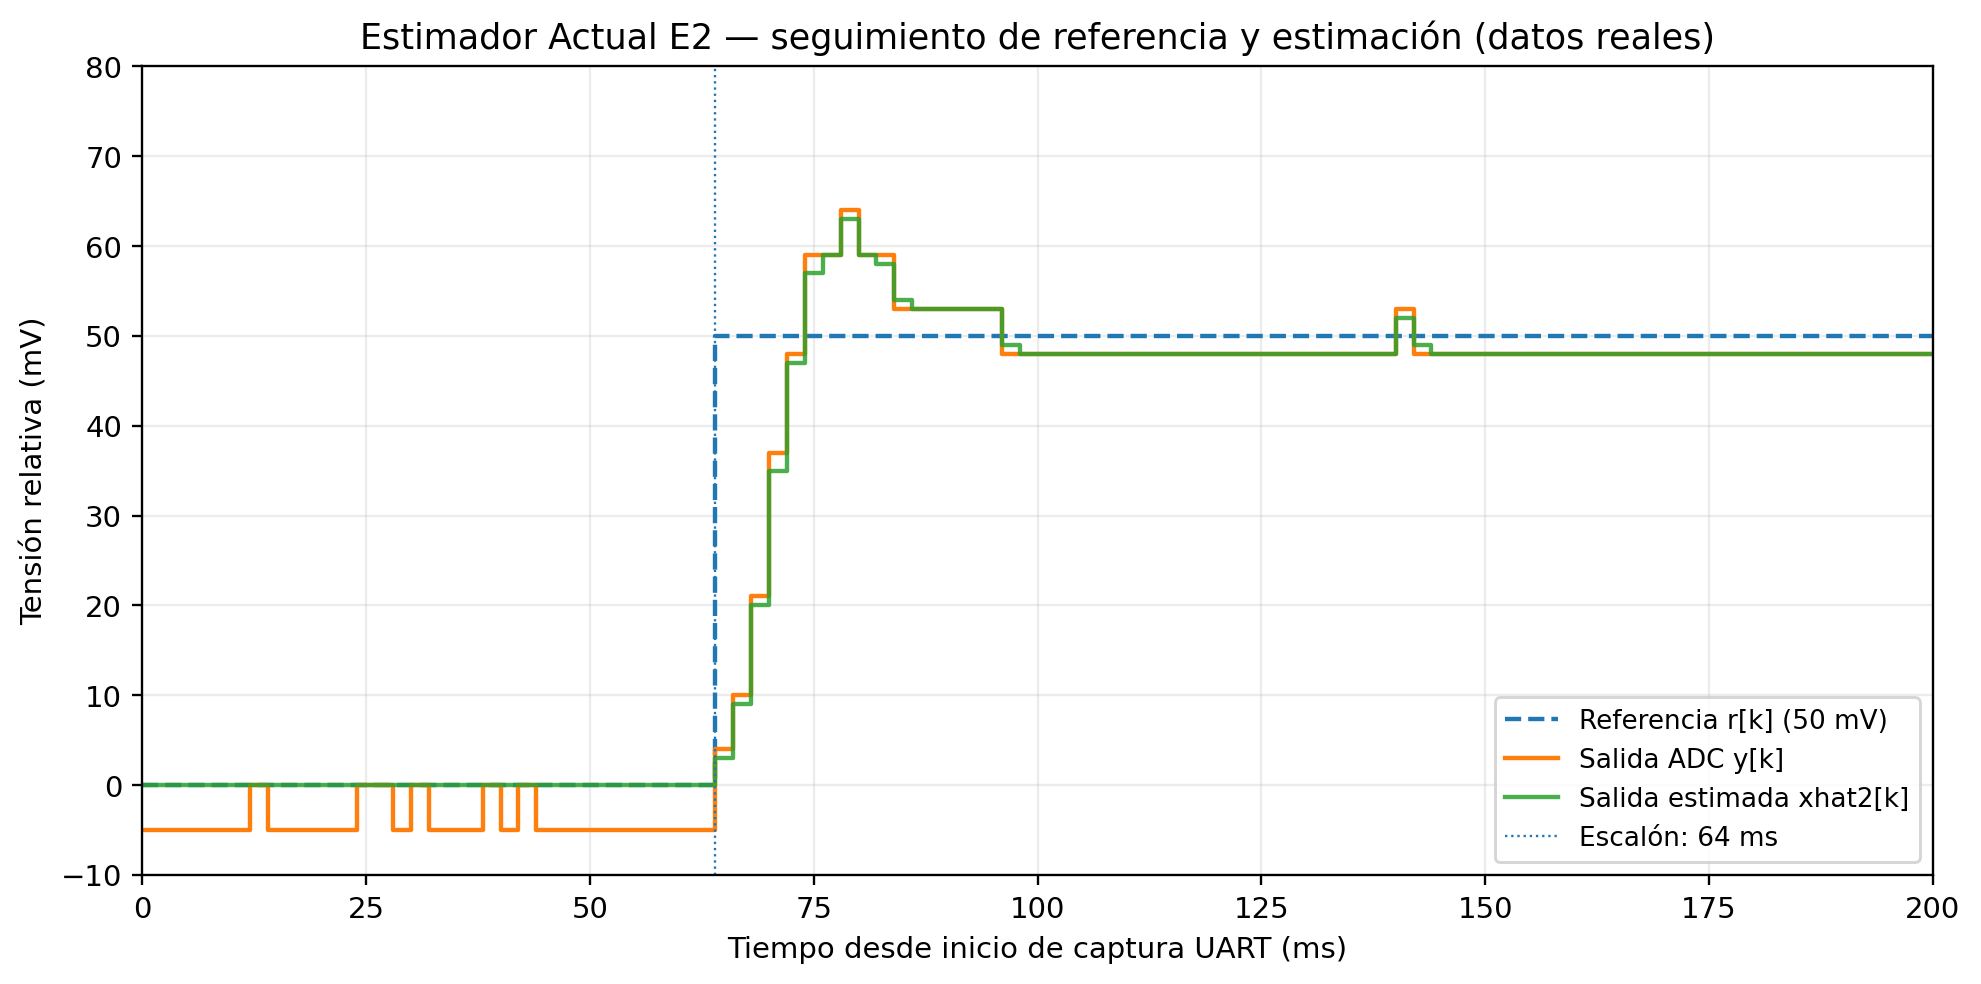
\includegraphics[width=\columnwidth]{01_actual_E2_salida_y_estimacion.png}
\caption{Actual E2: referencia, salida relativa y salida estimada registradas por el PSoC. La corrección actual se incorpora antes de calcular la acción de control.}
\label{fig:actual_e2_salida}
\end{figure}
\begin{figure}[!t]
\centering
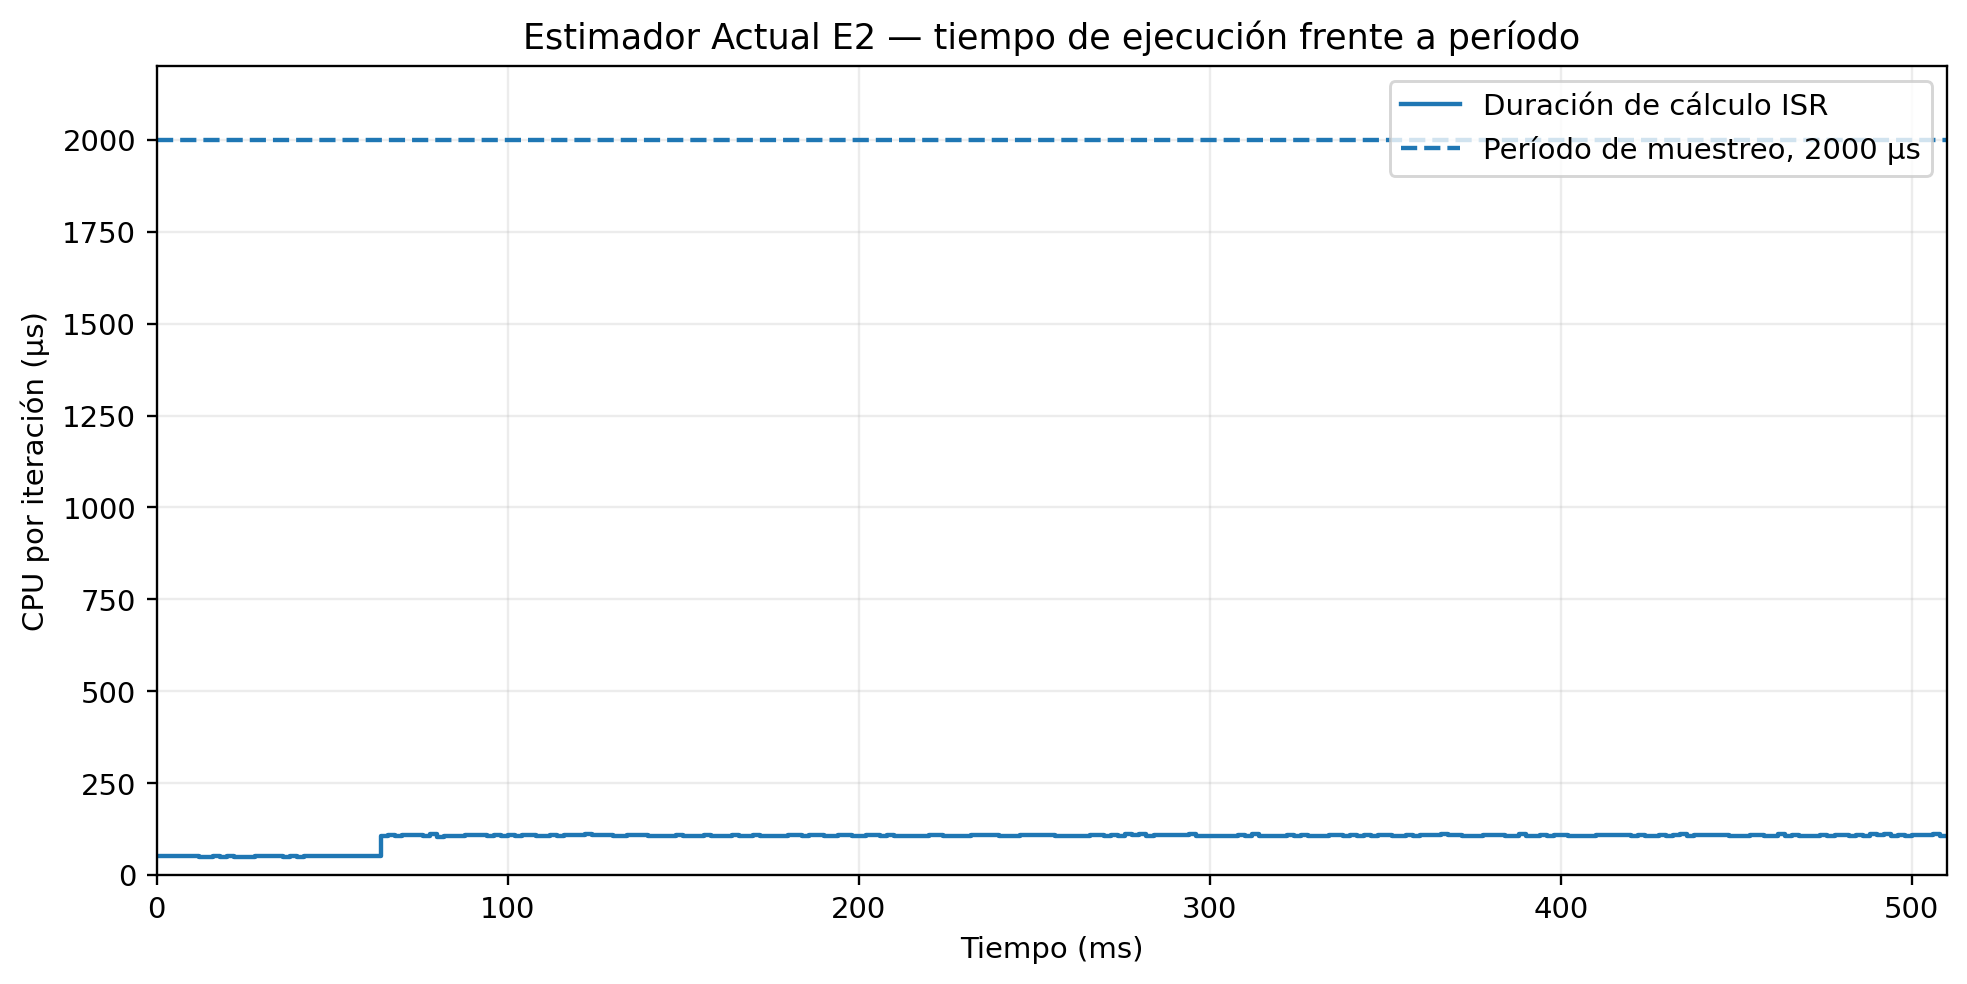
\includegraphics[width=\columnwidth]{04_actual_E2_tiempo_CPU.png}
\caption{Tiempo de cálculo de Actual E2 frente al período de muestreo de 2000 $\mu$s.}
\label{fig:cpu}
\end{figure}

En Actual E2 el RMS de \(y_{\mathrm{rel}}-\widehat y\) calculado desde el escalón fue \(0{,}366\,\mathrm{mV}\); para Predictor E2 se registraron \(1{,}473\,\mathrm{mV}\). Estos valores no miden directamente \(\|\boldsymbol{x}-\widehat{\boldsymbol{x}}\|\), ya que sólo se dispone de una salida física y el estado interno no se adquiere. Tampoco son estrictamente equivalentes entre arquitecturas: el estimador actual informa el estado ya corregido con la medida de la misma muestra, mientras que el predictor utiliza el estado anterior a la corrección.

En los cuatro casos, \(\max(\mathrm{CPU})\) quedó entre 110 y 112 $\mu$s, es decir, entre 5,5 y 5,6\,\% del intervalo de muestreo. Las 256 muestras de cada adquisición terminaron sin banderas activas, lo que constituye una comprobación de funcionamiento durante los \(0{,}51\,\mathrm{s}\) observados, aunque no equivale a una demostración de robustez general frente a perturbaciones no ensayadas.

\section{Discusión}
La diferencia entre los dos observadores es temporal: en la estructura actual, la medida modifica inmediatamente el estado que utiliza el control, mientras que en el predictor la innovación entra en la actualización de la muestra siguiente. La distinción explica que sus ganancias deban diseñarse con ecuaciones de error diferentes y que una misma ubicación de polos no produzca necesariamente la misma respuesta transitoria cuando se añaden incertidumbre, ruido y cuantización.

La evaluación sobre el modelo identificado obligó a revisar E1. El observador actual original, estable en la planta nominal, produjo \(\rho=1{,}0487\) con los parámetros identificados; el rediseño desplazó ese valor a \(0{,}8737\). En el predictor E1 alternativo resultó \(\rho\approx0{,}8550\); E2 conservó radios espectrales próximos a 0,83 en ambas arquitecturas. Esta comprobación fue determinante para no trasladar al laboratorio un diseño de control cuya estabilidad lineal dependía demasiado del modelo ideal.

Las mediciones reales muestran un matiz que no surge al observar únicamente las curvas de MATLAB: el mejor error medio de seguimiento por ADC corresponde a Actual E2 (4,24\,\% de la referencia), pero los incrementos físicos de J7 difieren sólo 0,41 mV entre las cuatro estructuras. La escala de referencia de 50 mV deja a la cuantización un peso considerable en la indicación de salida. Por ello, el valor de una muestra individual es menos significativo que el promedio de la meseta, y la atribución de diferencias pequeñas al observador exige ensayos repetidos con control de cero y ruido.

Finalmente, las cuatro imágenes del Rigol contienen el escalón, pero fueron tomadas con disparo forzado; en las capturas E1 y Actual E2 el modo esperado del programa de adquisición tampoco coincidió con el modo que confirmó la UART. Se mantuvieron sin alterar los archivos originales y se identificó esa limitación documental. El alineamiento por CH1 permite comparar tendencias y amplitudes, no afirmar que la diferencia entre picos temporales físicos sea inferior al período de registro. Del mismo modo, no se informa un tiempo de establecimiento estricto al 2\,\% respecto a 50 mV: la cuantización y el sesgo final impiden que todas las muestras permanezcan dentro de esa banda.

\section{Conclusiones}
Las cuatro configuraciones de realimentación de estados estimados pudieron implementarse sobre la misma planta analógica con \(T_s=2\,\mathrm{ms}\) y referencia de 50 mV. Cada ensayo registró 256 muestras sin banderas, con períodos medianos de 2000 $\mu$s y tiempos máximos de CPU entre 110 y 112 $\mu$s. El mando nominal no superó los 92 mV; ello deja margen frente a los límites conservadores establecidos en el firmware para estas ejecuciones.

El ensayo también mostró que la ubicación de polos debe comprobarse con el modelo efectivamente identificado y no sólo con el nominal. La configuración Actual E1 original alcanzó un radio espectral de 1,0487 sobre la planta identificada, mientras que su variante rediseñada lo redujo a 0,8737; con ella fue posible completar el ensayo físico sin observar divergencia en la ventana registrada. Los diseños E2 conservaron radios espectrales de 0,8288 y 0,8251, y ambos terminaron sin activar protecciones en la medición real.

Con la misma referencia, los predictores alcanzaron sobrepasamientos de 20 y 22\,\%, frente a 30 y 28\,\% de los estimadores actuales. La media final del ADC favoreció al Actual E2, con 47,88 mV y error medio de 2,12 mV, pero el Rigol midió incrementos finales de J7 entre 44,33 y 44,74 mV para todos los casos. Esta proximidad física, a pesar de las diferencias en UART, confirma que la resolución de la lectura y la corrección del cero condicionan la comparación del seguimiento a pequeña señal.

Para el montaje ensayado, los cuatro diseños permitieron reconstruir una salida estimada y ejecutar control digital sin exceder los límites registrados. La elección entre predictor y estimador actual no debe basarse en una sola cifra de error: el predictor mostró un menor pico de salida en estas pruebas, mientras que el actual corrigió la estimación con la muestra presente. Un estudio posterior con más repeticiones, sincronización de disparo físico y perturbaciones controladas permitiría cuantificar esa diferencia sin confundirla con la variabilidad instrumental. La experiencia reproduce una enseñanza central del control digital: la estabilidad del modelo discreto es indispensable, pero la valoración del sistema implementado exige observar también la conversión, el tiempo de cálculo y la señal analógica real.

\balance
\begin{thebibliography}{4}
\bibitem{samanta2024} B. Samanta, \emph{Introduction to Digital Control: An Integrated Approach}. Springer, 2024.
\bibitem{fadali2020} M. S. Fadali y A. Visioli, \emph{Digital Control Engineering: Analysis and Design}, 3.\textsuperscript{a} ed. Academic Press, 2020.
\bibitem{astrom2020} K. J. \AA str\"om y R. M. Murray, \emph{Feedback Systems: An Introduction for Scientists and Engineers}, 2.\textsuperscript{a} ed. Princeton University Press, 2021.
\bibitem{guiaLab7} C\'atedra de Automatizaci\'on, \emph{Utilizaci\'on y evaluaci\'on de estimadores de estado de predicci\'on y actual}, gu\'ia de pr\'actica, Universidad Cat\'olica ``Nuestra Se\~nora de la Asunci\'on'', 2026.
\end{thebibliography}
\end{document}
